
% Save this content as a .tex file and compile with a LaTeX editor (e.g., Overleaf)- https://www.overleaf.com/project/693c554b91da4cf891bc42ee

\documentclass[12pt,a4paper]{article}
\usepackage[utf8]{inputenc}
\usepackage{geometry}
\geometry{left=2.5cm, right=2.5cm, top=2.5cm, bottom=2.5cm}
\usepackage[table]{xcolor}
\usepackage{graphicx}
\usepackage{tikz}
\usetikzlibrary{shapes.geometric, arrows.meta, positioning, er, trees, backgrounds, fit, calc}
\usepackage{pgfgantt}
\usepackage{tabularx}
\usepackage{forest}
\usepackage{float}
\usepackage[hidelinks]{hyperref}
\usepackage{caption}

% Global TikZ Styles
\tikzset{
    startstop/.style={rectangle, rounded corners, minimum width=3cm, minimum height=1cm, text centered, draw=black, fill=red!30},
    process/.style={rectangle, minimum width=3cm, minimum height=1cm, text centered, draw=black, fill=orange!30},
    decision/.style={diamond, minimum width=3cm, minimum height=1cm, text centered, draw=black, fill=green!30, aspect=2},
    arrow/.style={thick,->,>=Stealth},
    entity/.style={rectangle, draw=black, fill=gray!30, minimum width=2.5cm, minimum height=1cm},
    datastore/.style={cylinder, shape border rotate=90, draw=black, fill=yellow!20, aspect=0.25, minimum width=2cm, minimum height=1cm}
}

\title{\textbf{Pharmacy Inventory Management System (IMS) \\ Project Report}}
\author{Developed by Pharmacy IMS Team}
\date{\y}

\begin{document}

\maketitle

\vspace{2cm}

\begin{center}
    \Large \textbf{Project Source Code} \\[1cm]
    \includegraphics[width=10cm]{qrcode_github.com.png} \\[1cm]
    \url{https://github.com/uzzal-portfolio/Pharmacy_IMS}
\end{center}
\newpage
\tableofcontents
\newpage

\section{Introduction}
The \textbf{Pharmacy Inventory Management System (IMS)} is an open-source web application designed to democratize pharmacy automation. Released under the **GNU General Public License v3.0**, this project embraces the spirit of "free software"—free to run, study, change, and share. Unlike proprietary systems locked behind expensive licenses, our IMS is built on a "primal stack" of \textbf{HTML, CSS, JavaScript, and PHP}. These core technologies are the backbone of the web and are widely understood by developers globally. This strategic choice ensures that the codebase remains accessible, allowing students, hobbyists, and business owners to easily clone the repository and tailor the system to their specific needs without a steep learning curve. By leveraging the power of open source, we aim to provide a robust, flexible, and cost-effective solution for modernizing pharmacy operations while fostering a community of collaborative improvement.

\section{Motivation}
The primary motivation for this project drives from the belief that essential business tools should be accessible to everyone. Many existing inventory systems are either prohibitively expensive or too complex to modify. We wanted to create a solution that breaks down these barriers. By using a foundational technology stack (HTML/PHP/MySQL), we ensure that even developers with basic knowledge can maintain and enhance the system. This "easy-to-modify" architecture empowers users to clone the project and adapt it for unique workflows, whether for a small local pharmacy or a large retail chain, ensuring true technological freedom and adaptability.


\section{Technical Specification}
This section outlines the architectural and strategic decisions that form the foundation of the Pharmacy IMS.

\subsection{Technical Perspective}
The system architecture follows a classic **Model-View-Controller (MVC)** inspired pattern, implemented using raw PHP for transparency and ease of modification.
\begin{enumerate}
    \item \textbf{Frontend}: Built with **Bootstrap 4** and **jQuery**, providing a responsive and interactive user interface without the complexity of heavy frontend frameworks.
    \item \textbf{Backend}: Core logic is written in **Vanilla PHP (v7.4+)**. This ensures compatibility with almost any standard web hosting environment.
    \item \textbf{Database}: **MySQL** is used for data persistence, interacting via **PDO (PHP Data Objects)** to ensure security against SQL injection.
    \item \textbf{Architecture}:
    \begin{itemize}
        \item \textbf{Modular Design}: Features like Inventory, Sales, and Reports are separated into distinct modules.
        \item \textbf{RBAC}: A robust Role-Based Access Control system restricts unauthorized access.
        \item \textbf{Security}: Input validation, session management, and password hashing (bcrypt) are strictly implemented.
    \end{itemize}
\end{enumerate}

\subsection{Business Perspective}
From a business standpoint, the system is designed to minimize operational costs while maximizing efficiency.
\begin{enumerate}
    \item \textbf{Cost-Effectiveness}: Being open-source eliminates licensing fees, making it ideal for small to medium independent pharmacies.
    \item \textbf{Scalability}: The modular database design allows for easy addition of new branches or features (e.g., e-commerce integration) in the future.
    \item \textbf{Reliability}: Automated calculations for sales and stock levels reduce human error, preventing revenue leakage.
    \item \textbf{Compliance}: The expiry tracking feature ensures no expired medication is sold, protecting the business from legal liabilities and maintaining customer trust.
\end{enumerate}

\section{Analysis \& Design}

\subsection{System Flow Chart}
\begin{figure}[H]
\centering
\resizebox{!}{0.8\textheight}{% Resize to fit height
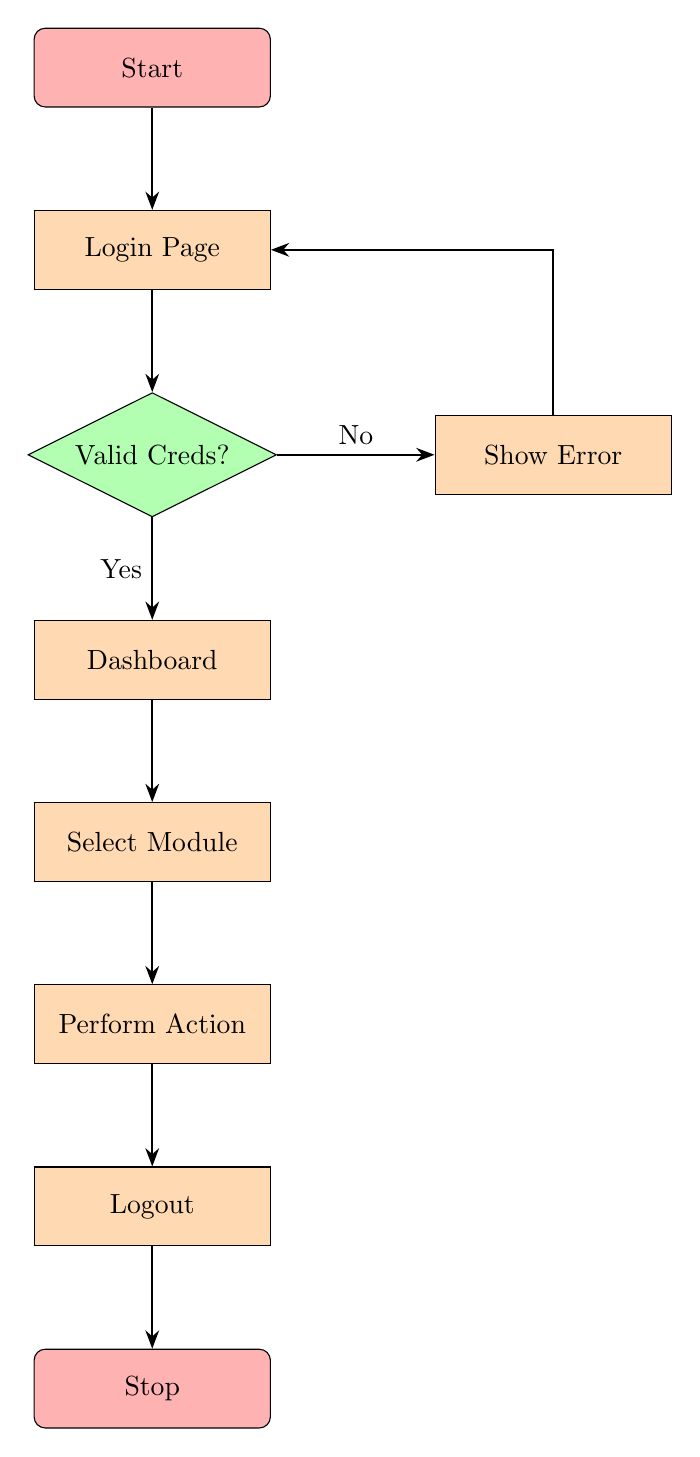
\begin{tikzpicture}[node distance=1.3cm and 1.3cm]
    \node (start) [startstop] {Start};
    \node (login) [process, below=of start] {Login Page};
    \node (decide) [decision, below=of login] {Valid Creds?};
    \node (dashboard) [process, below=of decide] {Dashboard};
    \node (error) [process, right=2cm of decide] {Show Error};
    
    \node (module) [process, below=of dashboard] {Select Module};
    \node (action) [process, below=of module] {Perform Action};
    \node (logout) [process, below=of action] {Logout};
    \node (stop) [startstop, below=of logout] {Stop};

    \draw [arrow] (start) -- (login);
    \draw [arrow] (login) -- (decide);
    \draw [arrow] (decide) -- node[anchor=east] {Yes} (dashboard);
    \draw [arrow] (decide) -- node[anchor=south] {No} (error);
    \draw [arrow] (error) |- (login);
    \draw [arrow] (dashboard) -- (module);
    \draw [arrow] (module) -- (action);
    \draw [arrow] (action) -- (logout);
    \draw [arrow] (logout) -- (stop);
\end{tikzpicture}
}
\caption{System Flow Chart}
\end{figure}

\subsection{Data Flow Diagrams (DFD)}

\subsubsection{Level 0 DFD (Context Diagram)}
\begin{figure}[H]
\centering
\includegraphics[width=0.9\textwidth]{DFD0.png}
\caption{Level 0 DFD}
\end{figure}

\subsubsection{Level 1 DFD (Inventory Module)}
\begin{figure}[H]
\centering
\includegraphics[width=0.9\textwidth]{DFD1.png}
\caption{Level 1 DFD}
\end{figure}

\newpage
\subsection{Decision Tree (Access Control)}
\begin{figure}[H]
\centering
\resizebox{\textwidth}{!}{
\begin{forest}
  for tree={l sep=1.5cm, s sep=1cm, edge={->, thick}, draw, rounded corners, inner sep=8pt, align=center, font=\sffamily}
  [Start Login
    [Check Credentials
      [Valid
        [Check Role
            [Admin
                [Access All Features, fill=green!20]
            ]
            [Store Clerk
                [Access POS \\ \& Inventory, fill=yellow!20]
            ]
            [Report Viewer
                [Access Reports \\ Only, fill=yellow!20]
            ]
        ]
      ]
      [Invalid
        [Show Error, fill=red!20]
      ]
    ]
  ]
\end{forest}
}
\caption{Access Control Decision Tree}
\end{figure}

\subsection{Decision Table (Role Permissions)}
\begin{table}[H]
\centering
\resizebox{\textwidth}{!}{
\begin{tabular}{|l|c|c|c|c|}
\hline
\textbf{Features / Roles} & \textbf{Admin} & \textbf{Store Clerk} & \textbf{Report Viewer} \\ \hline
Manage Inventory & \textbf{Yes} & \textbf{Yes} & No \\ \hline
Process Sales (POS) & \textbf{Yes} & \textbf{Yes} & No \\ \hline
View Reports & \textbf{Yes} & No & \textbf{Yes} \\ \hline
Manage Users & \textbf{Yes} & No & No \\ \hline
Manage Customers & \textbf{Yes} & No & No \\ \hline
\end{tabular}
}
\caption{System Access Control Matrix}
\end{table}

\subsection{Entity Relationship Diagram (ERD)}
\begin{figure}[H]
\centering
\resizebox{\textwidth}{!}{
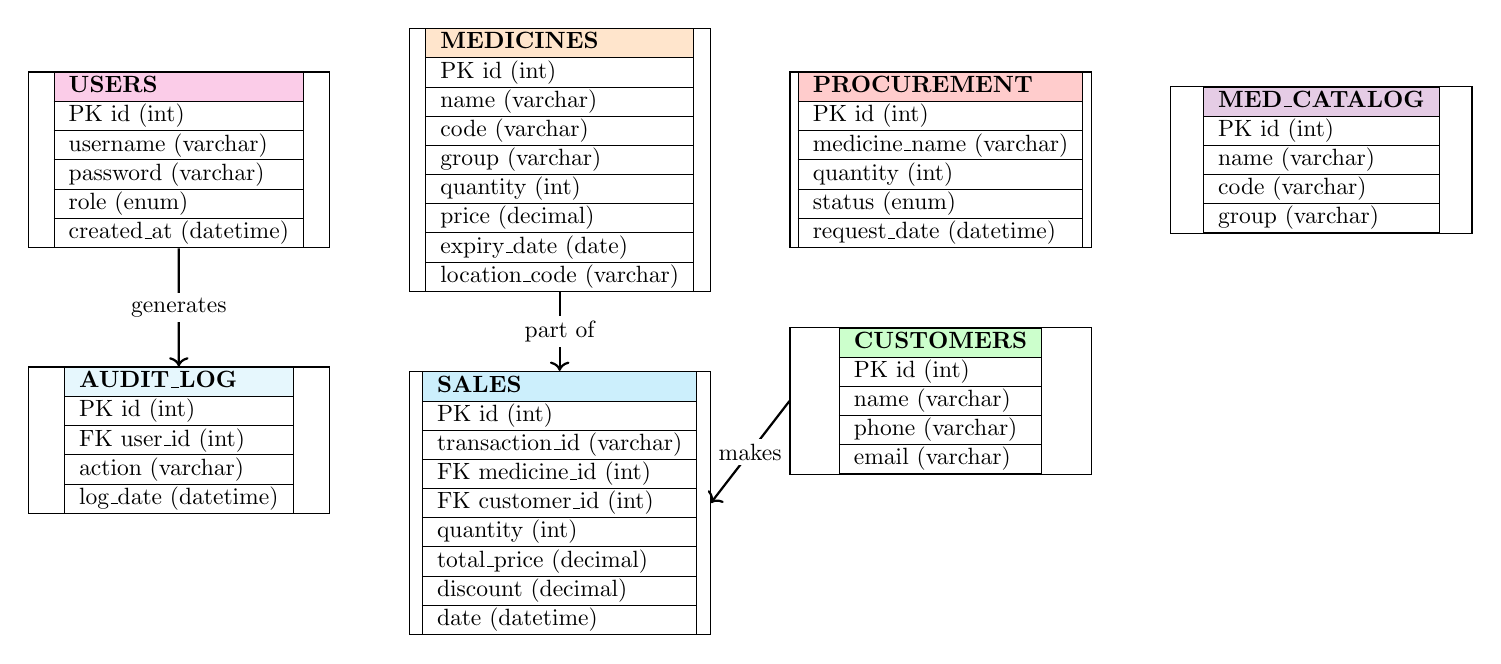
\begin{tikzpicture}[
    node distance=2cm, 
    every node/.style={scale=0.85},
    entity/.style={
        shape=rectangle,
        draw,
        fill=white,
        inner sep=0pt,
        text width=4.5cm,
        align=center
    }
]

    % USERS Table
    \node (users) [entity] {
        \begin{tabular}{|l|}
            \hline
            \rowcolor{magenta!20} \textbf{USERS} \\ \hline
            PK id (int) \\ \hline
            username (varchar) \\ \hline
            password (varchar) \\ \hline
            role (enum) \\ \hline
            created\_at (datetime) \\ \hline
        \end{tabular}
    };

    % AUDIT_LOG Table
    \node (audit) [entity, below=1.5cm of users] {
        \begin{tabular}{|l|}
            \hline
            \rowcolor{cyan!10} \textbf{AUDIT\_LOG} \\ \hline
            PK id (int) \\ \hline
            FK user\_id (int) \\ \hline
            action (varchar) \\ \hline
            log\_date (datetime) \\ \hline
        \end{tabular}
    };

    % MEDICINES Table
    \node (medicines) [entity, right=1cm of users] {
        \begin{tabular}{|l|}
            \hline
            \rowcolor{orange!20} \textbf{MEDICINES} \\ \hline
            PK id (int) \\ \hline
            name (varchar) \\ \hline
            code (varchar) \\ \hline
            group (varchar) \\ \hline
            quantity (int) \\ \hline
            price (decimal) \\ \hline
            expiry\_date (date) \\ \hline
            location\_code (varchar) \\ \hline
        \end{tabular}
    };

    % SALES Table
    \node (sales) [entity, below=1cm of medicines] {
        \begin{tabular}{|l|}
            \hline
            \rowcolor{cyan!20} \textbf{SALES} \\ \hline
            PK id (int) \\ \hline
            transaction\_id (varchar) \\ \hline
            FK medicine\_id (int) \\ \hline
            FK customer\_id (int) \\ \hline
            quantity (int) \\ \hline
            total\_price (decimal) \\ \hline
            discount (decimal) \\ \hline
            date (datetime) \\ \hline
        \end{tabular}
    };

    % PROCUREMENT Table
    \node (procurement) [entity, right=1cm of medicines] {
        \begin{tabular}{|l|}
            \hline
            \rowcolor{red!20} \textbf{PROCUREMENT} \\ \hline
            PK id (int) \\ \hline
            medicine\_name (varchar) \\ \hline
            quantity (int) \\ \hline
            status (enum) \\ \hline
            request\_date (datetime) \\ \hline
        \end{tabular}
    };

    % CUSTOMERS Table
    \node (customers) [entity, below=1cm of procurement] {
        \begin{tabular}{|l|}
            \hline
            \rowcolor{green!20} \textbf{CUSTOMERS} \\ \hline
            PK id (int) \\ \hline
            name (varchar) \\ \hline
            phone (varchar) \\ \hline
            email (varchar) \\ \hline
        \end{tabular}
    };

    % MEDICINE_CATALOG Table
    \node (catalog) [entity, right=1cm of procurement] {
        \begin{tabular}{|l|}
            \hline
            \rowcolor{violet!20} \textbf{MED\_CATALOG} \\ \hline
            PK id (int) \\ \hline
            name (varchar) \\ \hline
            code (varchar) \\ \hline
            group (varchar) \\ \hline
        \end{tabular}
    };

    % Relationships
    \draw [->, thick] (users) -- node[midway, fill=white, inner sep=2pt] {generates} (audit);
    \draw [->, thick] (medicines) -- node[midway, fill=white, inner sep=2pt] {part of} (sales);
    \draw [->, thick] (customers.west) -- node[midway, fill=white, inner sep=2pt] {makes} (sales.east);

\end{tikzpicture}
}
\caption{Entity Relationship Diagram (Database Schema)}
\end{figure}

\subsection{Gantt Chart (3 Month Timeline)}
\begin{figure}[H]
\centering
\resizebox{\textwidth}{!}{
\begin{ganttchart}[
    vgrid,
    hgrid,
    time slot format=isodate,
    x unit=0.3cm, % Compressing width
    y unit chart=0.7cm
    ]{2024-01-01}{2024-03-31}
    \gantttitlecalendar{year, month=name, week} \\
    
    \ganttgroup[progress=100]{Analysis}{2024-01-01}{2024-01-31} \\
    \ganttbar[progress=100]{Reqs}{2024-01-01}{2024-01-14} \\
    \ganttbar[progress=100]{Design}{2024-01-15}{2024-01-31} \\
    
    \ganttgroup[progress=80]{Implementation}{2024-02-01}{2024-02-29} \\
    \ganttbar[progress=100]{DB Setup}{2024-02-01}{2024-02-07} \\
    \ganttbar[progress=90]{Backend}{2024-02-08}{2024-02-21} \\
    \ganttbar[progress=70]{Frontend}{2024-02-15}{2024-02-29} \\

    \ganttgroup[progress=0]{Testing}{2024-03-01}{2024-03-31} \\
    \ganttbar{QA Tests}{2024-03-01}{2024-03-14} \\
    \ganttbar{Docs}{2024-03-15}{2024-03-25} \\
    \ganttbar{Release}{2024-03-26}{2024-03-31}
\end{ganttchart}
}
\caption{Project Timeline}
\end{figure}



\section{User Manual}
The User Manual provides a step-by-step guide to navigating and utilizing the key features of the Pharmacy IMS.

\subsection{Login Page}
\textbf{URL}: \url{http://localhost/Pharmacy_IMS/public/login.php}
\begin{figure}[H]
\centering
\includegraphics[width=0.9\textwidth]{LoginPage.png}
\caption{Login Page Screenshot}
\end{figure}
\begin{itemize}
    \item Enter your unique \textbf{Username} and \textbf{Password}.
    \item Click \textbf{Login}.
    \item If credentials are valid, you are redirected to the Dashboard based on your role (Admin, Clerk, or Viewer).
\end{itemize}

\subsection{Dashboard}
\textbf{URL}: \url{http://localhost/Pharmacy_IMS/public/welcome.php}
\begin{itemize}
    \item View total stats: Total Medicines, Total Sales, Expiring Soon.
    \item Quick links to main modules: Inventory, POS, Procurement, Reports.
\end{itemize}

\begin{figure}[H]
\centering
\includegraphics[width=0.9\textwidth]{heroPage.png}
\caption{Dashboard Screenshot}
\end{figure}

\subsection{Inventory Management}
\textbf{URL}: \url{http://localhost/Pharmacy_IMS/public/inventory.php}
\subsubsection{Add New Medicine}
\begin{enumerate}
    \item Click \textbf{Add New Medicine}.
    \item \textbf{Medicine Name}: auto-complete enabled to prevent duplicates.
    \item \textbf{Medicine Code}: Unique code. System alert if code already exists.
    \item \textbf{Group}: Categorize medicine (e.g., Tablet, Syrup).
    \item Fill Quantity, Price, Expiry Date, and Location.
    \item Click \textbf{Add Medicine}.
\end{enumerate}

\begin{figure}[H]
\centering
\includegraphics[width=0.9\textwidth]{inventory.png}
\caption{Inventory Management Screenshot}
\end{figure}

\subsection{Point of Sale (POS)}
\textbf{URL}: \url{http://localhost/Pharmacy_IMS/public/pos.php}
\begin{itemize}
    \item \textbf{Select Customer}: Search by Name or Phone number.
    \item \textbf{New Customer}: If not found, simply type the new name and proceed. The system auto-creates the profile.
    \item \textbf{Add Items}: Search medicine by Name or Code.
    \item \textbf{Expiry Check}: System blocks adding expired items to the cart.
    \item \textbf{Checkout}: Review cart, apply discounts, and complete sale.
\end{itemize}

\begin{figure}[H]
\centering
\includegraphics[width=0.9\textwidth]{pos.png}
\caption{Point of Sale (POS) Screenshot}
\end{figure}

\subsection{Customer Management}
\textbf{URL}: \url{http://localhost/Pharmacy_IMS/public/customer_database.php}
\begin{enumerate}
    \item \textbf{Add Customer}: Enter Name (Required).
    \item \textbf{Phone/Email}: Optional fields for quick entry.
    \item \textbf{Validation}: Phone field accepts only digits and '+' (max 15 chars).
\end{enumerate}

\begin{figure}[H]
\centering
\includegraphics[width=0.9\textwidth]{cdm.png}
\caption{Customer Management Screenshot}
\end{figure}

\subsection{Procurement}
\textbf{URL}: \url{http://localhost/Pharmacy_IMS/public/procurement.php}
\begin{itemize}
    \item \textbf{Request Stock}: Search for medicine by Name or Code. The form auto-fills the name.
    \item \textbf{Quantity}: Enter required amount.
    \item \textbf{Status}: Track requests as Pending, Approved, or Rejected.
\end{itemize}

\begin{figure}[H]
\centering
\includegraphics[width=0.9\textwidth]{pm.png}
\caption{Procurement Screenshot}
\end{figure}

\subsection{Reports}
\textbf{URL}: \url{http://localhost/Pharmacy_IMS/public/reports.php}
Select a report type to generate a structured PDF:
\begin{itemize}
    \item \textbf{Stock Report}: Current inventory status.
    \item \textbf{Sales Report}: Detailed financial logs.
    \item \textbf{Expiry Report}: List of medicines expiring soon.
    \item \textbf{Procurement Report}: Log of stock requests.
\end{itemize}

\begin{figure}[H]
\centering
\includegraphics[width=0.9\textwidth]{rep.png}
\caption{Reports Screenshot}
\end{figure}

\section{Dependencies and Requirements}
\subsection{Software Requirements}
\begin{itemize}
    \item \textbf{Web Server}: Apache HTTP Server (via XAMPP v7.4+ recommended).
    \item \textbf{Database}: MySQL or MariaDB.
    \item \textbf{Language}: PHP 7.4 or higher.
    \item \textbf{Browser}: Modern web browser (Chrome, Firefox, Edge).
\end{itemize}

\subsection{Hardware Requirements}
\begin{itemize}
    \item \textbf{Processor}: Intel Core i3 or equivalent.
    \item \textbf{RAM}: 4GB Minimum (8GB Recommended).
    \item \textbf{Storage}: 500MB free disk space for application and database.
\end{itemize}

\subsection{Deployment Network Diagram}
\begin{figure}[H]
\centering
\resizebox{0.8\textwidth}{!}{
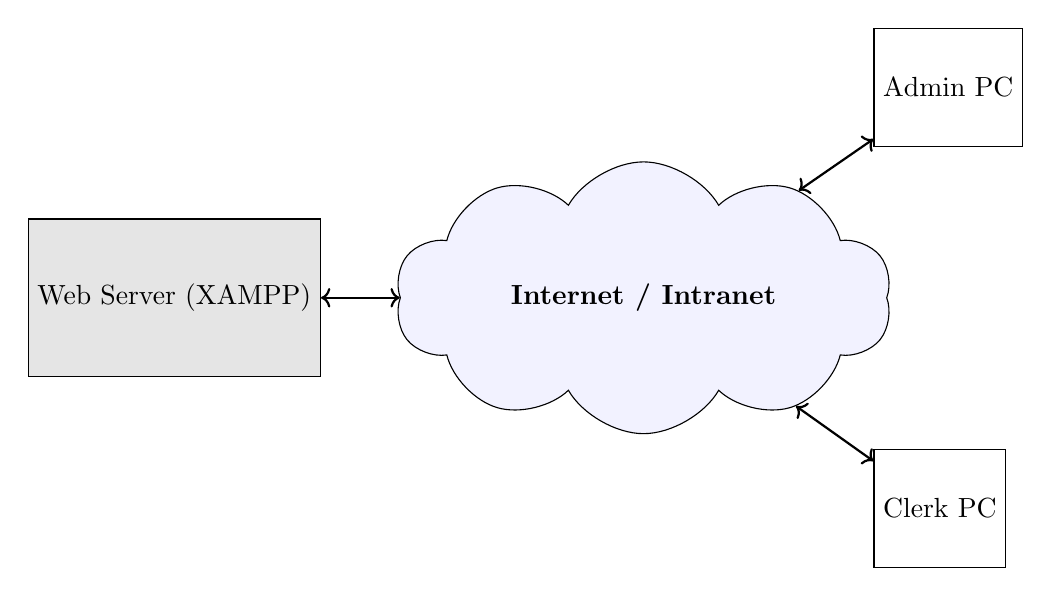
\begin{tikzpicture}[node distance=4cm]
    \node (cloud) [cloud, draw, cloud puffs=10, cloud puff arc=120, aspect=2.5, inner sep=0.5cm, fill=blue!5] {\textbf{Internet / Intranet}};
    
    \node (server) [rectangle, draw, fill=gray!20, minimum size=2cm, left=1cm of cloud] {Web Server (XAMPP)};
    
    \node (client1) [rectangle, draw, minimum size=1.5cm, above right=1cm of cloud] {Admin PC};
    \node (client2) [rectangle, draw, minimum size=1.5cm, below right=1cm of cloud] {Clerk PC};

    \draw [<->, thick] (server) -- (cloud);
    \draw [<->, thick] (cloud) -- (client1);
    \draw [<->, thick] (cloud) -- (client2);
\end{tikzpicture}
}
\caption{Deployment Network Diagram}
\end{figure}

\section{Conclusion}
The Pharmacy Inventory Management System successfully achieves its goal of digitizing and automating key pharmacy operations. By providing a robust platform for inventory control, sales processing, and reporting, the system minimizes manual errors and enhances operational efficiency. The modular design with Role-Based Access Control ensures security and scalability. Future enhancements could include cloud integration, barcode scanner support, and advanced predictive analytics for stock procurement, further solidifying its value as an essential tool for modern pharmacy management.

\end{document}